\documentclass[10pt]{standalone}
\usepackage[utf8]{inputenc}
\usepackage{pgfplots}
\pgfplotsset{compat=1.15}
\usepackage{mathrsfs}
\usetikzlibrary{arrows}
\pagestyle{empty}
\begin{document}
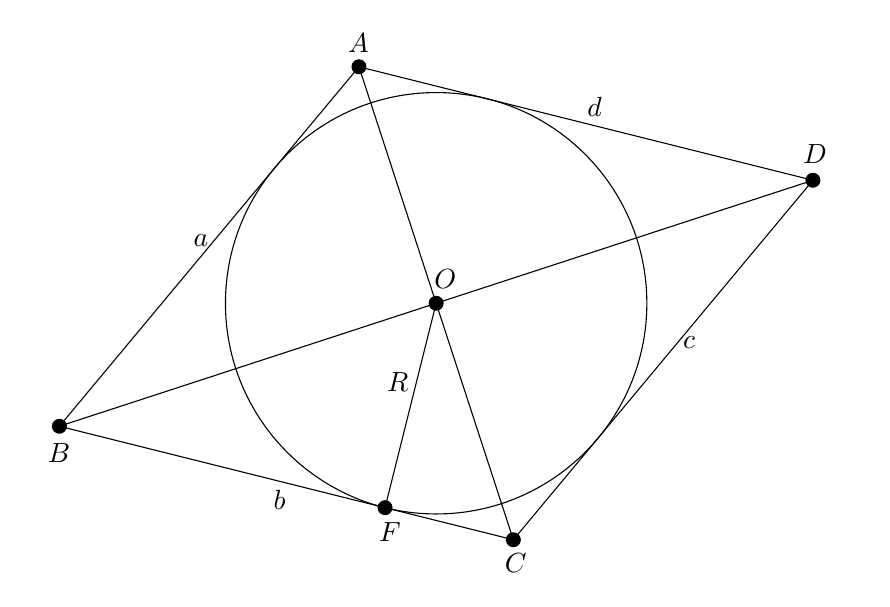
\begin{tikzpicture}[line cap=round,line join=round,>=triangle 45,x=1.0cm,y=1.0cm]
\clip(0.8,-3.5) rectangle (11.4,3.5);
\draw (5.987605034277024,0.) circle (2.6758696403846773cm);
\draw (5.007178340212068,3.003329965438631)-- (10.772477648234933,1.562005138432915);
\draw (10.772477648234933,1.562005138432915)-- (6.96803172834198,-3.003329965438631);
\draw (6.96803172834198,-3.003329965438631)-- (1.2027324203191148,-1.5620051384329152);
\draw (1.2027324203191148,-1.5620051384329152)-- (5.007178340212068,3.003329965438631);
\draw (5.007178340212068,3.003329965438631)-- (5.987605034277024,0.);
\draw (5.987605034277024,0.)-- (1.2027324203191148,-1.5620051384329152);
\draw (5.987605034277024,0.)-- (5.338611318530579,-2.5959748629857815);
\draw (5.987605034277024,0.)-- (6.96803172834198,-3.003329965438631);
\draw (5.987605034277024,0.)-- (10.772477648234933,1.562005138432915);

\draw [fill=black] (5.987605034277024,0.) circle (2.5pt);
\draw[color=black] (6.103656675060752,0.3042035220820447) node {$O$};
\draw [fill=black] (5.338611318530579,-2.5959748629857815) circle (2.5pt);
\draw[color=black] (5.4,-2.9) node {$F$};
\draw [fill=black] (5.007178340212068,3.003329965438631) circle (2.5pt);
\draw[color=black] (5.0,3.3) node {$A$};
\draw [fill=black] (10.772477648234933,1.562005138432915) circle (2.5pt);
\draw[color=black] (10.8,1.9) node {$D$};
\draw [fill=black] (6.96803172834198,-3.003329965438631) circle (2.5pt);
\draw[color=black] (7.0,-3.3) node {$C$};
\draw [fill=black] (1.2027324203191148,-1.5620051384329152) circle (2.5pt);
\draw[color=black] (1.2,-1.9) node {$B$};
\draw[color=black] (8.0,2.5) node {$d$};
\draw[color=black] (9.2,-0.5) node {$c$};
\draw[color=black] (4.0,-2.5) node {$b$};
\draw[color=black] (3.0,0.8) node {$a$};
%\draw[color=black] (5.291295189574655,1.5641927648768088) node {$q$};
%\draw[color=black] (3.5505205778187334,-0.375527516794078) node {$r$};
\draw[color=black] (5.5,-1.0) node {$R$};
%\draw[color=black] (6.269444733323222,-1.4365710896738795) node {$t$};
%\draw[color=black] (8.50758351986655,0.6855160560857234) node {$a$};

\end{tikzpicture}
\end{document}